We  now discuss   syntax and semantics of  our specifications, and illustrate through examples.

\subsection{Specifications Syntax }

Our specification language % \SpecLang,  
 supports scoped invariants,   method specifications, and {conjunctions}. 
\begin{definition} [Specifications]  { } %  We define the \emph{syntax} of \SpecLang and well-frmedness:
\noindent

\begin{itemize}
\item
The syntax of specifications, $S$, is given below
\label{f:holistic-syntax}
\[
\begin{syntax}
\syntaxElement{S}{ }
		  {\syntaxline
                               %   {  \OneStateQ {\overline {x:C}} {A} }	
				{ \TwoStatesN {\overline {x:C}} {A}  }
				%  {\mprepost{A}{C}{m}{x}{C}{A} }
%		 \endsyntaxline
% 		}
%  		{
% 		\syntaxline
 				{\mprepostN{A}{p\ C}{m}{y}{C}{A} {A}}%{A[\!\![ \,C\!::\!m(\overline{x:C})\,]\!\!] A }}
				{S\, \wedge \, S}
		 \endsyntaxline
 		}
\endSyntaxElement\ 
\syntaxElement{p}{ } 
 	 {\syntaxline
                                  {\  \ \ \  \prg{private} \ } 	
				 {\   \prg{public} \ } 	
		 \endsyntaxline
 		}
\endSyntaxElement 
\end{syntax}
\]

\item
{\emph{Well-formedness}},  $\vdash S$,  is   defined by cases on $S$:\\
  $\strut \ \  \vdash {\TwoStatesN {\overline {x:C}} {A}} \ \ \ \triangleq\  \ \ \fv(A)\subseteq\{  \overline x \}\,\wedge\, {M \vdash \encaps {\sdN{\overline {x: C}} \wedge A}} $;\\
 $\strut \ \  \vdash {\mprepostN{A}{p\ C}{m}{y}{C}{A'} {A''}}\ \ \ \triangleq\  \ \  \exists \overline x, \overline {C'}.[ $\\
  $\strut \hspace{1cm}  \sdN{\prg{res}\notin \overline{x}, \overline{y}}\,  \wedge\,  \ \sdN{\fv(A_0)\subseteq \overline{x},\overline y, \prg{this}}\   \wedge \fv(A')\subseteq  \fv(A),\prg{res}\   \wedge\  \fv(A'')\subseteq  \sdN{\overline{x}} $\\
  $\strut \hspace{1cm}\wedge\  \Pos A\, \wedge\, \Pos {A'}\, \wedge \,\Pos {A''}\, \wedge  \,  M \vdash \encaps  {\overline {x: C'} \wedge A''}\ \ \  ]$ \\
  $\strut \ \   \vdash S\, \wedge \, S' \ \ \triangleq \ \  \vdash S\, \wedge\, \vdash S'  $.  

\end{itemize} 
\end{definition}

{
 \begin{example}[Scoped Invariants]
 \label{example:twostate}
  % 
 $S_5$  guarantees   that   non-null keys do not change:
 \\
 \begin{tabular}{lcll}
$\strut \ \ \ \ \ \ \ \ S_5$ & $\triangleq$   & ${\TwoStatesN {\prg{a}:\prg{Account}.\prg{k}:\prg{Key}}  {\prg{null}\neq \prg{k}=\prg{a.\password}}} $  \end{tabular}
 \end{example} 
 }

 \begin{example}[Method Specifications]
 \label{example:mprepostl}
 A method specification for method \prg{buy} appeared in \S\ref{sec:howThird}. 
%  $S_6$ guarantees that  \prg{buy} does not decrease  the balance of the shop's account if its key is protected from the buyer, while 
Specification  $S_9$    guarantees that \prg{set} preserves the protectedness of any account, as well as of any key.  
%  Appendix~\ref{app:spec} contains further examples.

%   \small   {
%  {\sprepost
%		{\strut \ \ \ \ \ \ \ \ \ S_6} 
%		{   \protectedFrom{\prg{this}.\prg{\myAccount}.\prg{key}} {\prg{buyer}} \wedge \prg{this}.\prg{\myAccount}.\prg{\balance}=b
%		 }
%		{\prg{public Shop}} {\prg{buy}} {\prg{buyer}:\prg{external}, \prg{anItem}:\prg{Item} }
%		{ 
%		  \protectedFrom{\prg{this}.\prg{\myAccount}.\prg{key}} {\prg{buyer}} \wedge \prg{this}.\prg{\myAccount}.\prg{\balance}\geq b
%		 }}
%  }
%  \\
%  \small {
   {\sprepost
		{\strut \ \ \ \ \ \ \ \ \ S_9} 
		{  a:\prg{Account}, a':\prg{Account}\wedge  \inside{a}\wedge  \inside{a'.\prg{key}} }
		{\prg{public Account}} {\prg{set}} {\prg{key'}:\prg{Key}}
		{   \inside{a}\wedge  \inside{a'.\prg{key}}  }
		{   \inside{a}\wedge  \inside{a'.\prg{key}} }
}

Note that in $S_9$ the variables $a$, $a'$ are disjoint from \prg{this} and the formal parameters of \prg{set}. 
In that sense, $a$ and $a'$ are universally quantified; a call of \prg{set} will preserve protectedness for \emph{ all} accounts and their keys. %, whether locally  accessible or not.
% $S_9$ guarantees that any call of \prg{set} will preserve protractedness for all
\end{example}
 



\label{ssect:sem}
\subsection{Specifications Semantics}
 
\footnoteSD{TODO motivate;
Here what we had: As discussed in \S \ref{s:approach}, 
{open world specifications need to be able to provide}
guarantees which hold
during execution of an internal, 
known, trusted module $M$ when linked together with any
unknown, untrusted, module $M_{ext}$. These guarantees need only hold 
when the external module is executing; we are not concerned if they are
temporarily broken by the internal module. Therefore, we are only interested in states where the
executing object (\prg{this}) is an external object. 
To express our focus on external states, we define the  \emph{external states semantics}, of the form 
$\reduction{M_{ext}}{M}{\sigma}{\sigma'}$, where $M_{ext}$ is the external
module, and $M$ is the internal module, and where we
collapse all internal steps into one single step.
}

  
We now move to the semantics of specifications:   $M \models S$ expresses that  module  $M$   satisfies a specification  $S$.  
{For this, we first define what it means for a state $\sigma$ to satisfy a triple of assertions:}

 
\begin{definition} \label{def:hoare:sem}
For modules $\Mtwo$, $M$, state $\sigma$, and assertions $A$, $A'$ and  $A''$, we define:
\begin{itemize}
\item
$ {\satAssertQuadruple  \Mtwo  M     {A} \sigma {A'} {A''} } \ \ \triangleq \ \ \forall \overline{z}, \overline{w}, \sigma',\sigma''.[
$  \\
$\strut \hspace{.2cm} M,  \sigma \models  {A} % \, \wedge\,    {\GRelevant {\overline \alpha}  \sigma} 
  \  \ \Longrightarrow$\\
 $\strut   \ \ \ \  \  \ \ \ \   [ \ \ \  {\leadstoBoundedStarFin { \Mtwo\madd M}{\sigma}  {\sigma'} }\ \ \Longrightarrow\ \   M,  \sigma' \models  \sdN{A'} %[\overline{\interpret \sigma z/z}] 
 \ \ \ \  ] \ \ \ \wedge$\\
 $\strut   \ \ \ \  \  \ \ \ \   [ \ \  \ {\leadstoBoundedStar  {\Mtwo\madd M}{\sigma}  {\sigma''} }\ \  \ \Longrightarrow\   \   M,  \sigma'' \models  {(\extThis \rightarrow A''[\sdN{\overline{\interpret \sigma z/z}}])}\ \ \  ] $\\
% $\strut \hspace{.2cm}$ where  $ \overline z= \fv(A)\!\setminus\! \vs(\sigma.\prg{cont}),\ \overline w=\fv(A)  \ \ \ ]$ %\ \ \ \  \ \ \ \  \ \  \ \ \ \  \ \ \ \ ]$
 $\strut \hspace{.2cm}$ where  $ \overline z=\fv(A)  \ \ \ ]$ %\ \ \ \  \ \ \ \  \ \  \ \ \ \  \ \ \ \ ]$
\end{itemize} 
\end{definition}


\begin{definition}  [Semantics of  Specifications]
We define $\satisfies{M}{{S}}$ by cases over$S$: % the three possible syntactic forms.

\label{def:necessity-semantics}

\begin{enumerate}
 \item
 $\satisfies{M}{\TwoStatesN {\overline {x:C}} {A}} \ \  \ \triangleq   \ \ \ {\forall   \Mtwo,  \sigma.[\ {\satAssertQuadruple  \Mtwo  M    {\extThis \wedge \overline {x:C} \wedge A} \sigma {A} {A} }\ ].}$
  \item
 $\satisfies{M} { \mprepostN {A_1}{p\ D}{m}{y}{D}{A_2} {A_3} }\  \ \ \   \triangleq    \ \ \ \forall   \Mtwo,  \sigma.[\ $    \\
$\strut  \ \ \   \ \ \ \ \ \ \ \ \   \   { \forall   y_0,\overline y, \sigma[ \ \ \ \sigma.\prg{cont}\txteq {u:=y_0.m(y_1,..y_n)} \ \ \Longrightarrow \ \ 
\satisfies  {M} {\quadruple  {A_1'} }   {\sigma}   {A_2' } {A_3' }  \  \ \  ]} $  \\
$\strut  \ \ \   \ \ \ \ \ \ \ \ \   \  \mbox{where}$\\
$\strut  \ \ \   \ \ \ \ \ \ \ \ \   \   A_1' \triangleq   y_0:D,{\overline {y:D}}   \wedge   A[y_0/\prg{this}],\  \  A_2' \triangleq A_2[u/res,y_0/\prg{this}],\ \ A_3' \triangleq A_3  \  ]$  
 \item
 $\satisfies{M}{S\, \wedge\, S'}$\ \ \  \ \ \  $\triangleq$  \  \ \  \   $\satisfies{M}{S}\ \wedge \ \satisfies{M}{S'}$
\end{enumerate}
\end{definition}


\footnoteSD{First bullet: This means that we require all objects to satisfy even if not locally relevant. Second Bullet: notice that we are asking for globally relevant objects}  
\footnoteSD{{TODO: Make an example that demonstrates the difference if in the second bullet we had asked for locally relevant objects ${\overline o}$.}}
\footnoteSD{{TODO Notice that we assume that $\overline x$ are not free in $A$ -- cf Barendregt convention.}}
\footnoteSD{TODO: explain why we did not require the stronger $\leadstoFin{M_{ext}\!\circ \!M}{\sigma}{\sigma'}$ rather than $\leadstoBoundedStar {M_{ext}\!\circ \!M}{\sigma}  {\sigma'}$.}


We demonstrate the meaning of ${\TwoStatesN {\overline {x:C}} {A}}$ in Fig. \ref{fig:illusrPreserve} where we refine the execution shown in Fig. \ref{fig:UpSemantics}, and take it that the pink states, \ie   ${\sigma_6}$-${\sigma_9}$ and $\sigma_{13}$-$\sigma_{17}$, and  $\sigma_{20}$, $\sigma_{21}$ are external, and the green states, \ie   ${\sigma_{10}}$,  ${\sigma_{11}}$,   ${\sigma_{12}}$,  ${\sigma_{18}}$, and  ${\sigma_{19}}$, are internal. 

{Appendix~\ref{app:spec} contains examples of the semantics of some of our specifications.}

 \begin{figure}[htb]
\begin{tabular}{|c|}
\hline  % \\
\resizebox{7.3cm}{!}{
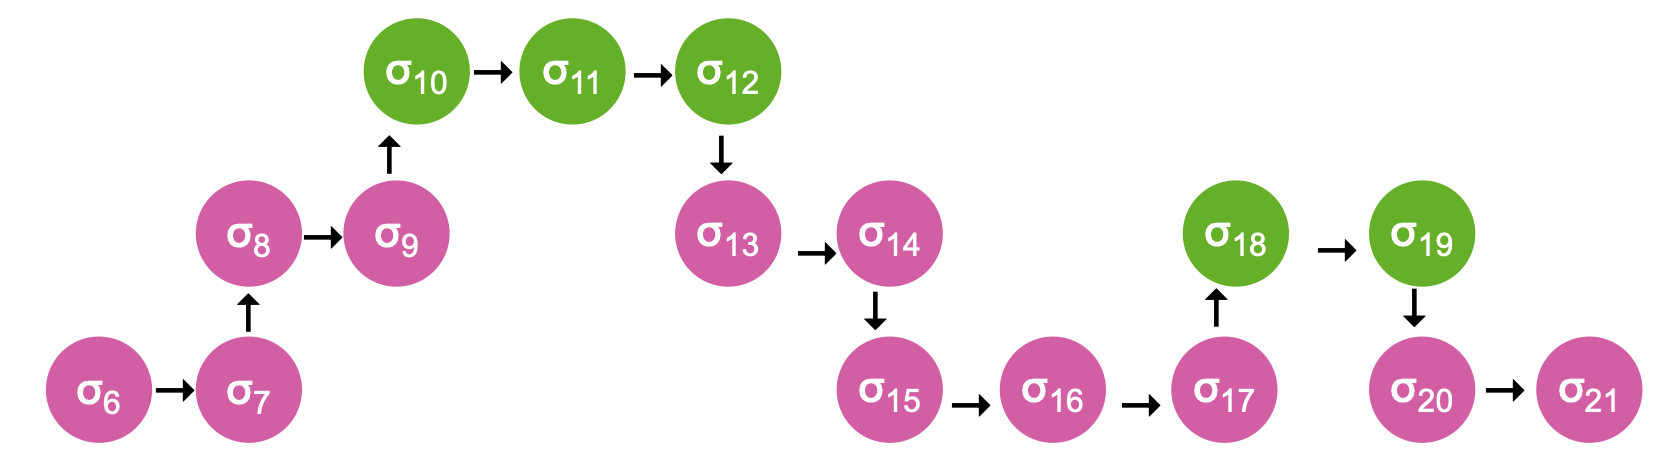
\includegraphics[width=\linewidth]{diagrams/preserves2.png}, 
}
\\
\hline
% \\
\begin{tabular}{lcl}
% not that interesting, chopped
% $\leadstoBoundedStar {...} {\sigma_6}   {\sigma_9} $ & &  $A_0$ guaranteed to be preserved from $\sigma_6$ to $\sigma_9$.\\
$\leadstoBoundedStar {...} {\sigma_6}   {\sigma_{13}} $ & &   $A_0$ guaranteed to be preserved from $\sigma_6$ to $\sigma_{13}$.\\
$\leadstoBoundedStar {...} {\sigma_6}   {\sigma_{19}} $, \ \   $..,\sigma_{19}\not \models {\extThis} $ & &   $A_0$ \emph{not} guaranteed to be preserved from $\sigma_6$ to $\sigma_{19}$.\\
$\leadstoBoundedStar {...} {\sigma_6}  {\sigma_{20}} $  \ \   & &  $A_0$  guaranteed to be preserved from $\sigma_6$ to $\sigma_{20}$.\\
$\notLeadstoBoundedStar {...} {\sigma_8}  {\sigma_{20}} $  \ \   & &  $A_0$  \emph{not} guaranteed to be preserved from $\sigma_8$ to $\sigma_{20}$. \\
\hline
\end{tabular}
\end{tabular}
   \caption{Illustrating  the meaning on ${\TwoStatesN {\overline {x:C}} {A_0}}$  -- refining Fig. \ref{fig:UpSemantics}. }
      \label{fig:illusrPreserve} 
 \end{figure}

%\move{
 %\begin{example}
 %\label{example:twostatesarisfy}
 %{We   revisit the specifications given in Sect. \ref{s:bankSpecEx}, and the one from Example \ref{example:twostate}, and  the three  modules from Sect. \ref{s:bank}:}
%
%
%\begin{tabular}{lllllllll}
%$\ModA  \models S_1$  &   $\ModA  \models S_2$ &  $\ModA \models S_3$ &   $\ModA \models S_4$    & $\ModA \models S_5$\\
% $\ModB \models S_1$  &   $\ModB \not\models S_2$   &  $\ModB  \models S_3$   &  $\ModB  \not\models S_4$   & $\ModB \not\models S_5$ \\
% $\ModC  \models S_1$    & $\ModC \models S_2$ &   $\ModC \models S_3$    &$\ModC \not\models S_4$   & $\ModC \not\models S_5$ 
%\end{tabular}
%\end{example}
 

 
 %\begin{example}
 %\label{example:mprepostlsatissy}
 %For  %method
 %Example \ref{example:mprepostl}, we have
 % $\ModA \models S_6$ and $\ModB \models S_6$ and  $\ModC \models S_6$.
%Also,  $\ModA \models S_7$ and $\ModB \models S_7$ and  $\ModC \models S_7$.
%However,   $\ModA  \models S_8$, while $\ModB  \not\models S_8$.
%\end{example}
%
 %\begin{example}
%\label{example:mprepostlsatissy}
 %For  %method
%any   specification  $S \triangleq {\mprepost{A}{p\ C}{m}{x}{C}{A'} }$ and any module  $M$ which does not have a class $C$  with a method $m$ with formal parameter  types ${\overline C}$, we have that $M \models S$.
%Namely, if a method were to be called with that signature on a $C$  from $M$, then execution would be stuck, and the requirements from Def. \ref{def:necessity-semantics}(3) would be trivially satisfied.
%Thus,   $\ModC \models S_8$. %, even though $\ModC$ does not have a method \prg{set} with the signature given in $S_6$;
%\end{example}
%}
 

%% KEEP ALL BELOW, but currently not needed 
%\subsection{\SpecLang Entailments}
%
%{We define entailment of specifications wrt a module in the expected way.} %The usual definition of entailment applies to our specifications as well}
%
%\begin{definition}[Satisfaction of Assertions by a module] 
%\label{def:assertion-inference-semantics}
%We define satisfaction of an assertion $A$ by a  module $M$ as:
%\begin{itemize}
%\item
%{
%$M \models A$   \ \ \ iff \ \ \  $\forall \overline{M}. \forall \sigma
%[\ \    \arising{\sigma}{M\madd\overline{M}}\   \  \wedge\ \  \satisfiesA {M}   {\sigma} {\external{\prg{this}}} 
%\   \ \Longrightarrow \ \ \satisfiesA{M}{\sigma}{A}\ \ ]$
%}\footnote{Not sure about the need for external and arising.}
%\end{itemize}
%\end{definition}
%
%%TODO: Here we will say that assertions are classical, as proven in FASE
%
%\begin{definition}[Stronger Specifications] 
%\label{def:specification-implication-semantics}
%Specification $S$ is stronger than another specification $S'$  in the context of a  module: 
% \begin{itemize}[itemsep=5pt]
%\item 
%$\stronger M  S  {S'}$   \ \ \ iff \ \ \  $M\models S$ implies $M \models S'$
%\item
%$\strongerEq M  S  {S'}$   \ \ \ iff \ \ \ $\stronger M  S  {S'}$  \ and \  $\stronger M   {S'} S$    
%\end{itemize}
%\end{definition}
%
%\noindent
%{Interestingly, entailment can deduce some method specifications out of two-state invariants.}
%
%{
% \begin{example}
% \label{example:entail}
% Any module $M$ whose code does not call  method \prg{buy} gives   $\stronger M {S_2 \wedge S_S4} {S_9}$
%\end{example}
%
%
%% Remember $S_1$, ... $S_4$ as defined in Sect. \ref{s:bankSpecEx}, and consider the specifications $S_6$ and $S_7$ from Example \ref{example:mprepostl}.
%% Then, for any module $M$ %which has a public method \prg{set}, 
%% we have that
%\begin{example}
% \label{example:entail}
%For any module $M$,  we have  $\strongerEq M {S_2 \wedge S_4} {S_2 \wedge S_{4a}}$, where $S_{4a}$ defined as 
%\\
%\begin{tabular}{lcll}
%  $S_{4a}$   & $\triangleq$   &  
% $ \TwoStatesQ{\prg{a}:\prg{Account},\prg{b}:\prg{int}}  {\inside{\prg{a.\password}} \wedge \prg{a.\balance}\geq\prg{b}} 
% {\inside{\prg{a.password}} \wedge \prg{a.\balance}\geq\prg{b}} $
% \end{tabular}
%\ \end{example}
%}
% 
%%Some properties of $M \models \_  \subseteq \_ $ are given below:
%%
%%\begin{lemma}
%%For assertions $A$, $A'$, variables $\overline y$, and $\overline x$, specifications $S$, $S'$, $S''$, and module $M$:
%%\begin{itemize} [topsep=6pt,itemsep=5pt,parsep=0pt,partopsep=0pt]
%%%\item
%%% $\stronger M {\OneStateQ {\overline {x:C}}  {A}}  {\TwoStatesQ {\overline {x:C}} {A}{A}} $ 
%%%    \item
%%%  $\strongerEq  M  {\OneStateQ    {y:\prg{Object}}   {\forall \overline {x:C}[ A ] } } 
%%%    {\OneStateQ {\overline {x:C}}  {A}} $.
%%\item
%%$\strongerEq M    {\TwoStatesQ {\overline {x:C}} {A}{A'}}    {\TwoStatesQ {\overline {y:C}} {A[y/x]}{A'[y/x]}}$
%%\item
%%$  M  \models    \overline {x:C} \wedge A_1'  \rightarrow A_1$ \ \ \  and \ \ \
%%$  M  \models  \overline {x:C} \wedge A_2'  \rightarrow A_2$  \ \ \ \ 
%%implies\\
%% $\strut \hspace{5cm} \stronger M  {\TwoStatesQ {\overline {x:C}} {A_1}{A_2}}     {\TwoStatesQ {\overline {x:C}} {A_1'}{A_2'}}$
%%
%%\item
%%$\stronger M  S {S''}$ and $\stronger M {S''} {S'}$\ \  \ implies\  \ \ $\stronger M S  {S'}$.
%%
%%\end{itemize}
%%
%%\end{lemma}


%%%%%%%%%%%%%%%%%%%%%%%%%%%%%%%%%%%%%%%%%%%%%%%%%%%%%%%%%%%%%%%%%%%%%%


